\let\negmedspace\undefined
\let\negthickspace\undefined
\documentclass[journal,12pt,twocolumn]{IEEEtran}
\usepackage{gensymb}
\usepackage{amssymb}
\usepackage[cmex10]{amsmath}
\usepackage{amsthm}
\usepackage[export]{adjustbox}
\usepackage{bm}
\usepackage{longtable}
\usepackage{enumitem}
\usepackage{mathtools}
\usepackage[breaklinks=true]{hyperref}
\usepackage{listings}
\usepackage{color}                                            %%
\usepackage{array}                                            %%
\usepackage{longtable}                                        %%
\usepackage{calc}                                             %%
\usepackage{multirow}                                         %%
\usepackage{hhline}                                           %%
\usepackage{ifthen}                                           %%
\usepackage{lscape}     
\usepackage{multicol}
% \usepackage{enumerate}
\DeclareMathOperator*{\Res}{Res}
\renewcommand\thesection{\arabic{section}}
\renewcommand\thesubsection{\thesection.\arabic{subsection}}
\renewcommand\thesubsubsection{\thesubsection.\arabic{subsubsection}}
\renewcommand\thesectiondis{\arabic{section}}
\renewcommand\thesubsectiondis{\thesectiondis.\arabic{subsection}}
\renewcommand\thesubsubsectiondis{\thesubsectiondis.\arabic{subsubsection}}
\hyphenation{op-tical net-works semi-conduc-tor}
\def\inputGnumericTable{}                                 %%
\lstset{
frame=single, 
breaklines=true,
columns=fullflexible
}
\begin{document}
\newtheorem{theorem}{Theorem}[section]
\newtheorem{problem}{Problem}
\newtheorem{proposition}{Proposition}[section]
\newtheorem{lemma}{Lemma}[section]
\newtheorem{corollary}[theorem]{Corollary}
\newtheorem{example}{Example}[section]
\newtheorem{definition}[problem]{Definition}
\newcommand{\BEQA}{\begin{eqnarray}}
\newcommand{\EEQA}{\end{eqnarray}}
\newcommand{\define}{\stackrel{\triangle}{=}}
\bibliographystyle{IEEEtran}
\providecommand{\mbf}{\mathbf}
\providecommand{\pr}[1]{\ensuremath{\Pr\left(#1\right)}}
\providecommand{\qfunc}[1]{\ensuremath{Q\left(#1\right)}}
\providecommand{\sbrak}[1]{\ensuremath{{}\left[#1\right]}}
\providecommand{\lsbrak}[1]{\ensuremath{{}\left[#1\right.}}
\providecommand{\rsbrak}[1]{\ensuremath{{}\left.#1\right]}}
\providecommand{\brak}[1]{\ensuremath{\left(#1\right)}}
\providecommand{\lbrak}[1]{\ensuremath{\left(#1\right.}}
\providecommand{\rbrak}[1]{\ensuremath{\left.#1\right)}}
\providecommand{\cbrak}[1]{\ensuremath{\left\{#1\right\}}}
\providecommand{\lcbrak}[1]{\ensuremath{\left\{#1\right.}}
\providecommand{\rcbrak}[1]{\ensuremath{\left.#1\right\}}}
\theoremstyle{remark}
\newtheorem{rem}{Remark}
\newcommand{\sgn}{\mathop{\mathrm{sgn}}}
\providecommand{\abs}[1]{\left\vert#1\right\vert}
\providecommand{\res}[1]{\Res\displaylimits_{#1}} 
\providecommand{\norm}[1]{\left\lVert#1\right\rVert}
%\providecommand{\norm}[1]{\lVert#1\rVert}
\providecommand{\mtx}[1]{\mathbf{#1}}
\providecommand{\mean}[1]{E\left[ #1 \right]}
\providecommand{\fourier}{\overset{\mathcal{F}}{ \rightleftharpoons}}
%\providecommand{\hilbert}{\overset{\mathcal{H}}{ \rightleftharpoons}}
\providecommand{\system}{\overset{\mathcal{H}}{ \longleftrightarrow}}
	%\newcommand{\solution}[2]{\textbf{Solution:}{#1}}
\newcommand{\solution}{\noindent \textbf{Solution: }}
\newcommand{\cosec}{\,\text{cosec}\,}
\providecommand{\dec}[2]{\ensuremath{\overset{#1}{\underset{#2}{\gtrless}}}}
\newcommand{\myvec}[1]{\ensuremath{\begin{pmatrix}#1\end{pmatrix}}}
\newcommand{\mydet}[1]{\ensuremath{\begin{vmatrix}#1\end{vmatrix}}}
\numberwithin{equation}{subsection}
\makeatletter
\@addtoreset{figure}{problem}
\makeatother
\let\StandardTheFigure\thefigure
\let\vec\mathbf
\renewcommand{\thefigure}{\theproblem}
\def\putbox#1#2#3{\makebox[0in][l]{\makebox[#1][l]{}\raisebox{\baselineskip}[0in][0in]{\raisebox{#2}[0in][0in]{#3}}}}
     \def\rightbox#1{\makebox[0in][r]{#1}}
     \def\centbox#1{\makebox[0in]{#1}}
     \def\topbox#1{\raisebox{-\baselineskip}[0in][0in]{#1}}
     \def\midbox#1{\raisebox{-0.5\baselineskip}[0in][0in]{#1}}
\vspace{3cm}
\title{10th CBSE MATHEMATICS}
\author{2006-07}
\maketitle
\newpage
\bigskip
\renewcommand{\thefigure}{\theenumi}
\renewcommand{\thetable}{\theenumi}
\section{Section A}
\renewcommand{\theequation}{\theenumi}
\begin{enumerate}[label=\thesection.\arabic*.,ref=\thesection.\theenumi]
\numberwithin{equation}{enumi}
\item Solve for x and y: \\ 
\begin{enumerate}
    \item $47x + 31y = 63\\$\\
    $31x + 47y = 15\\$\\
    \item $\frac{ax}{b}  - \frac{by}{a}  = a+b$\\
    $ ax - by = 2ab $\\
\end{enumerate}
\item Given that P = $\frac{2}{x^2-x-6}$ , Q= $\frac{3}{x^2+x-3}$ , R = $\frac{4}{x^2-4x+3}$. Find (P + Q) + R\\
\vspace{5mm}\\
\item If $ (x-2)(x+3) $ is the HCF of the polynomials\\
\vspace{2mm}\\
$ P\myvec{x} = \myvec{x^2 - 3x + 2)(2x^2 + 7x + a}$  and\\
$ Q\myvec{x} = \myvec{x^2 + 4x + 3}{3x^2 - 7x + b}$\\
\vspace{2mm}\\
Find the values of $a$ and $b$\\
\vspace{5mm}\\
\item \begin{enumerate}
    \item Solve for $'x'$, $ 12abx^2 - \myvec{9a^2 - 8b^2} \cdot x - 6ab = 0 $\\
    \item A two-digit number is such that the product of its digits is 35. When 18 is added the number the digits interchange their places. Find the number\\
\end{enumerate}
\item The 6th term of an Arithmetic Progression (AP) is -10 and the term is -26. Determine the $15^{th}$ term of AP\\
\item Find the sum of all the two digit natural numbers which are divisible by 4.\\
\item A household article is available for Rs. 2,500 cash or Rs.520 cash down payment followed by four equal monthly installments.
If the rate of interest charged under the installment plan is 25\% per annum. Find the amount of each installment.\\
\item A man borrows Rs. 36,410 from a finance company and has to repay it in three equal annual installments. Find the amount of each
installment if the rate of interest is 10\% per annum compounded annually.\\
\item In Fig $\ref{fig1}$, $\angle{ACB} = 90^\circ , CD \perp AB $, prove that $CD^2 = BD \cdot AD $\\
\begin{figure}[h!]
    \centering
    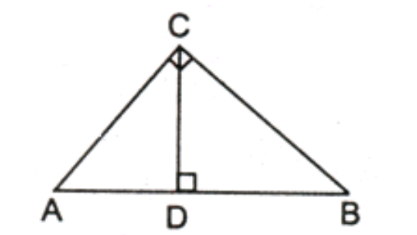
\includegraphics[width=0.5\columnwidth,center]{fig 1.1.png}
	\caption{}
	\label{fig1}
 \end{figure}
\vspace{2mm}
\item In Fig $\ref{fig2}$, $\vec{PA} = 3cm, \vec{AB} = 9, \vec{CD} = 5$\\
Find the length of PC\\
\begin{figure}[h!]
    \centering
    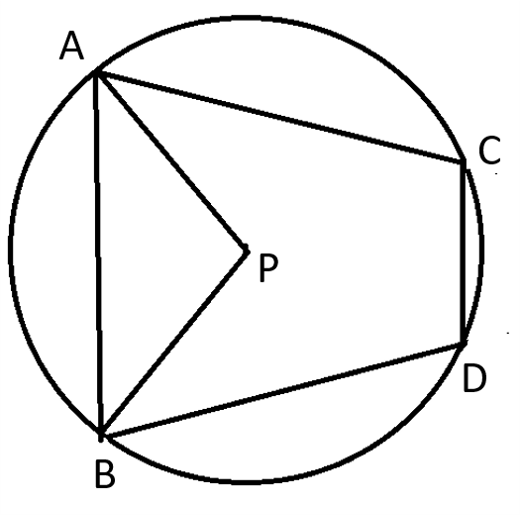
\includegraphics[width=0.5\columnwidth,center]{fig 1.2.png}
	\caption{}
	\label{fig2}
 \end{figure}
\end{enumerate}
\section{Section B}
\renewcommand{\theequation}{\theenumi}
\begin{enumerate}[label=\thesection.\arabic*.,ref=\thesection.\theenumi]
\numberwithin{equation}{enumi}
\item Draw the graphs of the equations\\
$ 4x - y - 8 = 0 $\\
$ 2x - 3y + 6 = 0 $\\
Also determine the vertices of the triangle formed by the lines and the
x axis\\
\item A train travels the distance of 300km in a uniform speed. If the speed
is increased by 5 kmph, the journey would have taken 2 hours less. Find the 
original speed of the train.\\
\item The radius of the base and the height of a solid right circular cylinder
are in the ratio of 2:3, and its volume is $\myvec{1617 cm^3}$. Find the total 
surface area of the cylinder. ( Use $\pi$  as  $\frac{22}{7} $ )\\
\item 
\begin{enumerate}
    \item  Prove that:\\
     \begin{align}
       \frac{\sin{\theta} + \cos{\theta}}{\sin{\theta} - \cos{\theta}}  + \frac{\sin{\theta} - \cos{\theta}}{\sin{\theta} + \cos{\theta}} = \frac{2 \sec^2 \theta}{\tan^2 \theta - 1} \nonumber
     \end{align}
     \item Evaluate the following without using the trigonometric tables:
     \begin{align}
     \frac{\sec^2\myvec{90^\circ - \theta} - \cot^2\theta}{\sin^2 25^\circ + \sin^2 65^\circ}
     \nonumber \\ + \frac{2\cos^2 60^\circ \tan^2 28^\circ tan^2 62^\circ}{3\myvec{sec^2 43^\circ - cot^2 47^\circ}} \nonumber
     \end{align}
\end{enumerate}

\item Construct a triangle ABC in which BC = 7cm, $\angle{A} = 60^\circ $  and altitude AD = 5cm. Write the steps of construction as well.\\

\item \begin{enumerate}
    \item Show that the points A = \myvec{1,2}, B \myvec{S,4}, C = \myvec{3,8}, D = \myvec{-1,6} are the vertices of a square\\
    \item Find the coordinates of the point equidistant from the 3 points given, A\myvec{5,1}, B\myvec{-3, -7}, C\myvec{7,-1}.\\
\end{enumerate}
\item Find the value of p for which the point \myvec{-1,3}, \myvec{2,p} and \myvec{5,-1} are collinear. \\

\item The Arithmetic mean of the following frequency distribution is 50. Find the value of p\\
\vspace{1mm}\\
\scalebox{0.8}{
\begin{tabular}{|l||c|c|c|c|c|}
    \hline
    Classes & 0-20 & 20-40 & 40-60 & 60-80 & 80-100  \\
    \hline\hline
    Frequency & 17 & p & 32 & 24 & 19\\
    \hline
\end{tabular}
}
\vspace{1mm}\\
\item The following table shows the monthly expenditure of a family
. Draw a Pie Chart for this data.\\
\vspace{2mm}\\
\scalebox{0.8}{
\begin{tabular}{|l||c|c|c|c|c|}
    \hline
    Item & Rent & Food & Clothing & Education & Misc.  \\
    \hline\hline
    Amount(Rs) & 1500 & 3600 & 1200 & 2100 & 2400\\
    \hline
\end{tabular}
}
\\
\item A box contains 20 balls bearing numbers 1,2,3....20. A ball is drawn at random from the box. What is the probability that the ball is\\
(a) an odd number\\
(b) divisible by 2 or 3 \\
(c) prime number\\
(d) not divisible by 10\\
\end{enumerate}
\section{Section C}
\renewcommand{\theequation}{\theenumi}
\begin{enumerate}[label=\thesection.\arabic*.,ref=\thesection.\theenumi]
\numberwithin{equation}{enumi}
\item Prove that the ratio of the areas of 2 similar triangles, is equal to the ratio
of the squares of their corresponding sides.Using the above, prove that the area of the
equilateral triangle described on the side of a right angled isosceles, is half the area
of an equilateral triangle described on its hypotenuse.\\
\item Prove that the angle subtended by an arc is double the angle subtended by it at any 
point, on the remaining part of the circle, Using the above, find $x$ in Fig $\ref{fig3}$
\begin{figure}[h!]
    \centering
    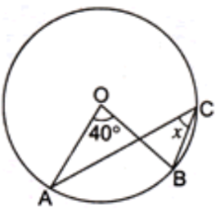
\includegraphics[width=0.5\columnwidth,center]{fig 1.3.png}
	\caption{}
	\label{fig3}
 \end{figure}
\item \begin{enumerate}
\item The rain water from a roof $22m \times 20m$ drains into a cylindrical vessel, having a diameter at the base of $2m$ and a height of $3.5m$. Lithe vessel is just full, find the rainfall in centimeters.\\
\item A bucket made up of a metal sheet is in the form of a frustum of a cone of height 16cm, with its radii of its lower and upper ends at 8 and 20 cm respectively, Find the cost of the bucket if the cost of the metal sheet used is Rs $15$ per $100 cm^2$. Use ($\pi$ as 3.14)\\
\end{enumerate}
\item \begin{enumerate}
\item The angles of depression of the top and the bottom of a building 50 meters high as observed from the top of a tower are $30^\circ$ and $60^\circ$ respectively. Find the height of the tower and also the horizontal distance between the building and the tower\\
\item The angle of elevation of the top of a tower is observed from a point on the ground as $\alpha$ and moving from that point the angle of elevation can be found to be $\beta$ metres towards the tower, the angle of elevation is $\theta$. Prove that the height of the tower is $( \frac{\tan \alpha \times \tan \beta}{\tan \beta - \tan \alpha})$ \\
\end{enumerate}
\item The annual income from the salary of Mrs. Usha, who is a senior citizen is Rs. 3,85,000, she donates Rs. 10,000 to the Prime Minister's relief fund ($100\%$ exemption), and another Rs. 10,000 to a Charitable Society ($50\%$ exemption), she contributes Rs. 70,000 to PFF annually, and pays a quartarly premium of Rs. 3,500 towards life insurance, She also purchases NSC's, for Rs. 20,000, she pays 1,600 per month towards income tax for 11 months. What is her tax liability ?\\
Use the following for calculating income tax:\\
1. Savings: $100\%$ exemption for savings upto Rs. 1,00,000\\
2. Rate of income tax for senior citizens\\
\vspace{1mm}\\
\scalebox{0.8}{
\begin{tabular}{|l||l|}
    \hline
    Slab & Income tax\\
    \hline\hline
     Upto Rs. 1,85,000 & No tax \\
     \hline
     From 1,85,001 to 2,50,000 & 20\% of taxable income \\
      & income above 1,85,000\\
      \hline
     From 2,50,001 and above & Rs 13000 + 30\% of the \\
       &  income exceeding\\
       & Rs 2,50,000\\
     \hline
\end{tabular}
}
\vspace{1mm}\\
3.Education cess: 2\% of  income tax\\
\end{enumerate}
\end{document}